\documentclass[11pt]{article}
\usepackage[backend=biber,natbib=true,style=authoryear]{biblatex}
\addbibresource{/home/nguyen/1_NQBH/reference/bib.bib}
\usepackage[utf8]{inputenc}
\usepackage{float}
\usepackage{graphicx}
\usepackage[colorlinks=true,linkcolor=blue,urlcolor=red,citecolor=magenta]{hyperref}
\usepackage{amsmath,amssymb,amsthm,mathtools}
\allowdisplaybreaks
\numberwithin{equation}{section}
\newtheorem{assumption}{Assumption}[section]
\newtheorem{lemma}{Lemma}[section]
\newtheorem{corollary}{Corollary}[section]
\newtheorem{definition}{Definition}[section]
\newtheorem{proposition}{Proposition}[section]
\newtheorem{theorem}{Theorem}[section]
\newtheorem{notation}{Notation}[section]
\newtheorem{remark}{Remark}[section]
\newtheorem{example}{Example}[section]
\newtheorem{ques}{Question}[section]
\newtheorem{problem}{Problem}[section]
\newtheorem{conjecture}{Conjecture}[section]
\usepackage[left=0.5in,right=0.5in,top=1.5cm,bottom=1.5cm]{geometry}
\usepackage{fancyhdr}
\pagestyle{fancy}
\fancyhf{}
\addtolength{\headheight}{0pt}% obsolete
\lhead{\small \textsc{Sect.} ~\thesection}
\rhead{\small \nouppercase{\leftmark}} %\nouppercase ! %\nouppercase !
\renewcommand{\sectionmark}[1]{\markboth{#1}{}}
\cfoot{\thepage}

\title{Report}
\author{Hong Nguyen}
\date{\today}

\begin{document}
\maketitle
\setcounter{secnumdepth}{6}
\tableofcontents

%------------------------------------------------------------------------------%

\section{Stationary Navier-Stokes equations}
In order to optimize the shape design of air ducts in combustion engines, we consider a shape optimization problem subject to a stationary incompressible viscous Navier-Stokes equations in 3D with appropriate physical boundary conditions in the duct geometry. An inflow profile is given at the inlet, a no-slip boundary condition is imposed on the wall, and a do-nothing boundary condition on the outlet. To find optimal shapes, we choose a mixed cost functional to achieve the flow uniformity at the outlet and minimize the dissipated power of our fluid dynamics device in a well balanced way.

To model the flow in the considered shape, we use the following initial boundary value problem for the stationary incompressible viscous Navier--Stokes equations:
\begin{equation}
    \label{NS}
    \tag{NS}
    \left\{\begin{split}
        -\nu\Delta{\bf u} + ({\bf u}\cdot\nabla){\bf u} + \nabla p &= {\bf f},&&\mbox{ in }\Omega,\\
        \nabla\cdot{\bf u} &= 0,&&\mbox{ in }\Omega,\\
        {\bf u} &= {\bf f}_{\rm in},&&\mbox{ on }\Gamma_{\rm in},\\
        {\bf u} &= {\bf 0},&&\mbox{ on }\Gamma_{\rm wall},\\
        -\nu\partial_{\bf n}{\bf u} + p{\bf n} &= {\bf 0},&&\mbox{ on }\Gamma_{\rm out}.
    \end{split}\right.
\end{equation}
Here, $\Omega\subset\mathbb{R}^N$ an open connected set, ${\bf u}:\Omega\to\mathbb{R}^N$ and $p:\Omega\to\mathbb{R}$ denote the \textit{velocity vector field} and the \textit{kinematic pressure}, respectively. We assume that the \textit{kinematic viscosity} $\nu > 0$ and the density of the external volume force ${\bf f}:\Omega\to\mathbb{R}^N$, the inflow profile ${\bf f}_{\rm in}:\Gamma_{\rm in}\to\mathbb{R}^N$ are given.

\begin{figure}[H]
    \centering
    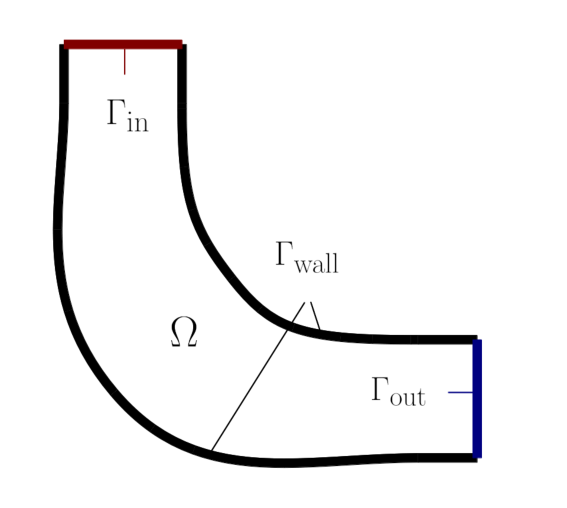
\includegraphics[width=0.35\textwidth]{geometry_simple_sketch}
    \caption{Simple sketch of a curved duct geometry.}
    \label{fig:geometry simple sketch}
\end{figure}

\subsection{Cost functionals}
The uniformity of the flow leaving the outlet is an important design criterion of automotive air ducts to enhance the efficiency of distributing the air flow \cite{Othmer2008}. To achieve this criterion, we minimize a cost functional capturing the distance between the normal component of the velocity and a given desired value of that quantity in the outlet:
\begin{align}
    \label{cost functional: outflow uniformity}
    \tag{$J_1$}
    J_1({\bf u},\Omega)\coloneqq\frac{1}{2}\int_{\Gamma_{\rm out}} \left({\bf u}\cdot{\bf n} - \overline{u}\right)^2{\rm d}\Gamma, \mbox{ where }\overline{u}\coloneqq -\frac{1}{H_{N-1}(\Gamma_{\rm out})}\int_{\Gamma_{\rm in}} \textbf{f}_{\rm in}\cdot{\bf n}{\rm d}\Gamma,
\end{align}
where $H_{N-1}(\Gamma_{\rm out})$ is the $(N - 1)$-dimensional \textit{Hausdorff measure} of the outflow $\Gamma_{\rm out}$.

Another criterion engineers also want to minimize is the power dissipated by air ducts (and any fluid dynamics devices in general) \cite{Othmer2008}. This dissipated power can be computed as the net inward flux of energy through the boundary of the considered tube:
\begin{align}
    \label{cost functional: energy dissipation}
    \tag{$J_2$}
    J_2({\bf u},p,\Omega)\coloneqq -\int_\Gamma \left(p + \frac{1}{2}|{\bf u}|^2\right){\bf u}\cdot{\bf n}{\rm d}\Gamma.
\end{align}
Concerning the regularity theory of Navier-Stokes equations with mixed boundary conditions (see, e.g., \cite{Mazya_Rossmann2007, Mazya_Rossmann2009}), the spatial components of its solutions $({\bf u},p)$ usually belong to the space $W^{1,2}(\Omega;\mathbb{R}^N)\times L^2(\Omega)$. Thus, the trace of $p$ on the boundary $\Gamma$ in the definition of $J_2({\bf u},p,\Omega)$ is not well-defined, and we consider the following approximation of $J_2({\bf u},p,\Omega)$, on account of the boundary condition on $\Gamma_{\rm wall}$, instead:
\begin{align}
    \label{cost functional: approximated energy dissipation}
    \tag{$J_2^\delta$}
    J_2^\delta({\bf u},p,\Omega)\coloneqq&\, -\frac{H_{N-1}(\Gamma_{\rm in})}{\operatorname{m}_N(\Gamma_{\rm in}^\delta)}\int_{\Gamma_{\rm in}^\delta} \left(p + \frac{1}{2}|{\bf u}|^2\right){\bf u}\cdot{\bf n}{\rm d}{\bf x} - \frac{H_{N-1}(\Gamma_{\rm out})}{\operatorname{m}_N(\Gamma_{\rm out}^\delta)}\int_{\Gamma_{\rm out}^\delta} \left(p + \frac{1}{2}|{\bf u}|^2\right){\bf u}\cdot{\bf n}{\rm d}{\bf x}\\
    =&\,\int_\Omega k_\delta({\bf x})\left(p + \frac{1}{2}|{\bf u}|^2\right){\bf u}\cdot{\bf n}{\rm d}{\bf x},\nonumber
\end{align}
where $\operatorname{m}_N$ denotes the $N$-dimensional \textit{Lebesgue measure} and
\begin{align*}
    k_\delta({\bf x})\coloneqq -\frac{H_{N-1}(\Gamma_{\rm in})}{\operatorname{m}_N(\Gamma_{\rm in}^\delta)}\chi_{\Gamma_{\rm in}^\delta}({\bf x}) - \frac{H_{N-1}(\Gamma_{\rm out})}{\operatorname{m}_N(\Gamma_{\rm out}^\delta)}\chi_{\Gamma_{\rm out}^\delta}({\bf x}),\ \forall{\bf x}\in\Omega.
\end{align*}

\begin{figure}[H]
    \centering
    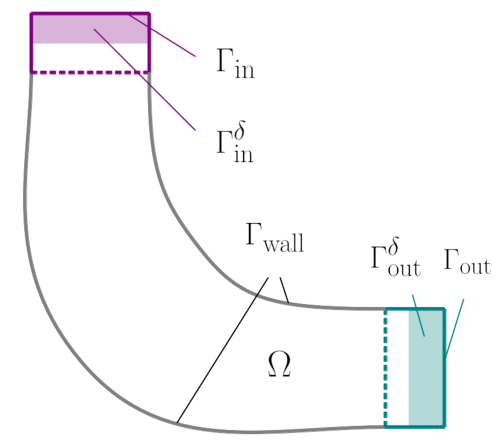
\includegraphics[width=0.35\textwidth]{./images/WIAS/geometry_delta}
    \caption{The duct geometry with $\delta$-approximated inlet $\Gamma_{\rm in}^\delta$ and $\delta$-approximated outlet $\Gamma_{\rm out}^\delta$.}
    \label{fig:geometry cutoff inlet outlet}
\end{figure}
Taking into account both objectives, we consider a mixed cost functional as a convex combination of the cost functionals above with a weighting parameter $\gamma\in[0,1]$:
\begin{align}
    \label{mixed cost functional}
    \tag{$J_{12}^{\delta,\gamma}$}
    J_{12}^{\delta,\gamma}({\bf u},p,\Omega)\coloneqq&\, (1 - \gamma)J_1({\bf u},\Omega) + \gamma J_2^\delta({\bf u},p,\Omega)\\
    =&\,\frac{1 - \gamma}{2}\int_{\Gamma_{\rm out}} \left({\bf u}\cdot{\bf n} - \overline{u}\right)^2{\rm d}\Gamma + \int_\Omega \gamma k_\delta({\bf x})\left(p + \frac{1}{2}|{\bf u}|^2\right){\bf u}\cdot{\bf n}{\rm d}{\bf x}.\nonumber
\end{align}
A typical PDE-constrained shape optimization problem (see, e.g., \cite{Delfour_Zolesio2011, Sokolowski_Zolesio1992}) can be established by finding an admissible shape to minimize the mixed cost functional under the given Navier-Stokes equation: Optimize $\Omega$ over an appropriate class of admissible domains, denoted by $\mathcal{O}_{\textrm{ad}}$, such that the mixed cost functional $J_{12}^{\delta,\gamma}({\bf u},p,\Omega)$ is minimized subject to \eqref{NS}, i.e.:
\begin{align}
    \label{shape optimization problem}
    \tag{sop}
    \min_{\Omega\in\mathcal{O}_{\textrm{ad}}} J_{12}^{\delta,\gamma}({\bf u},p,\Omega) \mbox{ such that } ({\bf u},p)\mbox{ solves \eqref{NS}}.
\end{align}

\section{Instationary Navier-Stokes equations}

\section{Smagorinsky turbulence models}

\section{$k$-$\epsilon$ turbulence models}
Standard $k$-$\epsilon$ turbulence model:
\begin{equation}
    \label{k-epsilon}
    \left\{\begin{split}
        \partial_t\overline{\bf u} - \nabla\cdot\left((\nu + \nu_{\rm t})\boldsymbol{\varepsilon}(\overline{\bf u})\right) + (\overline{\bf u}\cdot\nabla)\overline{\bf u} + \nabla\left(\overline{p} - \frac{2}{3}k\right) &= {\bf f},\\
        \nabla\cdot\overline{\bf u} &= 0,\\
        \partial_tk - \nabla\cdot\left(c_k\frac{k^2}{\epsilon}\nabla k\right)+ \overline{\bf u}\cdot\nabla k &= c_\nu\frac{k^2}{\epsilon}|\boldsymbol{\varepsilon}(\overline{\bf u})|^2 - \epsilon,\\
        \partial_t\epsilon - \nabla\cdot\left(c_\varepsilon\frac{k^2}{\epsilon}\nabla\epsilon\right) + \overline{\bf u}\cdot\nabla\epsilon &= c_\eta k|\boldsymbol{\varepsilon}(\overline{\bf u})|^2 - (c_{\varepsilon 2} - c_\gamma)\frac{\epsilon^2}{k},
    \end{split}\right.
\end{equation}
where $\nu_{\rm t}\coloneqq c_\nu\frac{k^2}{\epsilon}$.


%------------------------------------------------------------------------------%

\printbibliography[heading=bibintoc]
\end{document}